\justify

\chaptertitle{RESULTS AND DISCUSSION}

\section{Results}
While we focus mostly on the theoretical aspect of the problem, we
performed some experiment to visualize the algorithm.
We generated a dataset in $\R^2$ under the group weakly linear separable
condition, with $K=9$ classes and $L=3$ groups with margin $\gamma$,
shown in Fig~\ref{fig:data}.

\begin{figure}[hbt!]
\centering
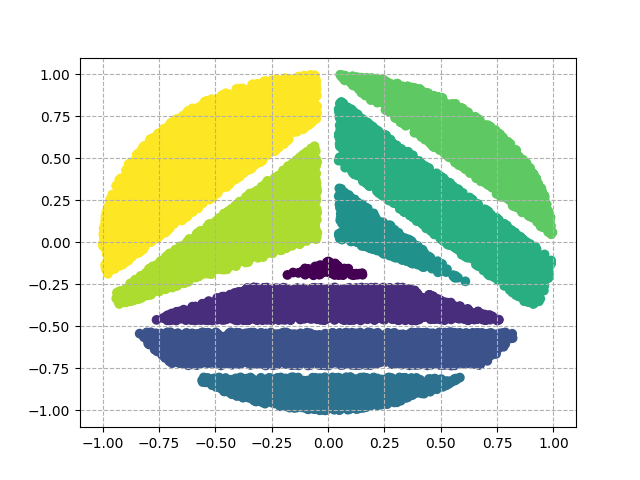
\includegraphics[width=0.5\textwidth]{weakly.png}
\caption{Group weakly separable dataset in $\R^2$.}
\label{fig:data}
\end{figure}

We compared two versions of the bandit multiclass perceptron~\cite{BeygelzimerPSTWZ2019-separable},
the standard one and the kernelized one (using the rational kernel).  Since the standard one only works with strongly separable case, it would definitely fail in this experiment, but we used it to give an overall sense of improvement for the kernelized version.  We ran both algorithms for $10^5$ steps for 5 times.  Fig.~\ref{fig:result} shows the result.  The kernelized version made on average $15831$ mistakes ($15.8\%$), while the standard one made on average $76759.4$ mistakes ($76.7\%$).  Theoretically, the kernelized version should stop making mistakes at some point, but since the number of steps that we ran is too low, we can only see that increasing rate of the number of mistakes decreases over time.

\begin{figure}[hbt!]
\centering
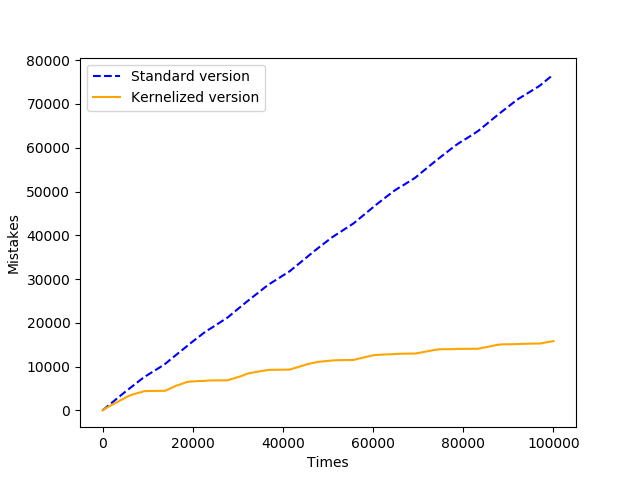
\includegraphics[width=0.5\textwidth]{result.png}
\caption{
Comparison of the standard algorithm and the kernelized algorithm with $T=10^5$.  
}
\label{fig:result}
\end{figure}

To see the decision boundary, we ploted the contours of the corresponding polynomials for two classes shown in Fig.~\ref{fig:bound_line1} and Fig.~\ref{fig:bound_line2}.  Note that the class in Fig.~\ref{fig:bound_line2} was much harder to learn as its boundary still overlapped with other classes (i.e., mistakes could still be made).

%\begin{figure}[h]
%\centering
%\includegraphics[width=0.5\textwidth]{Figure_1.png}
%\caption{Algorithm with rational kernel final decision boundaries}
%\label{fig:data-bound}
%\end{figure}

\begin{figure}[hbt!]
\centering
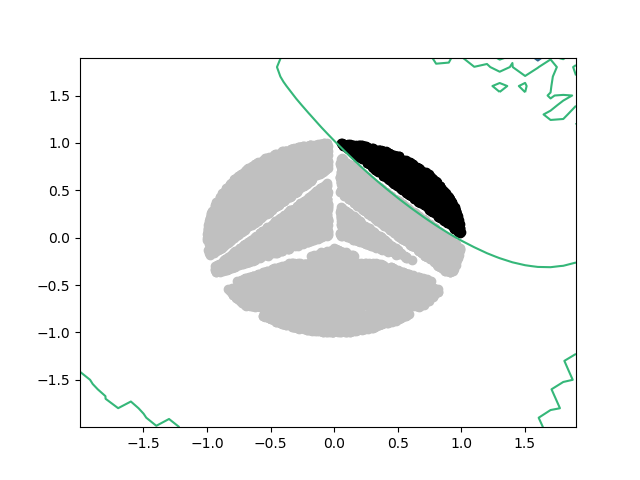
\includegraphics[width=0.5\textwidth]{Figure_7.png}
\caption{
The boundary line of a class (in black) of the kernelized algorithm after $T=10^5$ steps. 
}
\label{fig:bound_line1}
\end{figure}

\begin{figure}[hbt!]
\centering
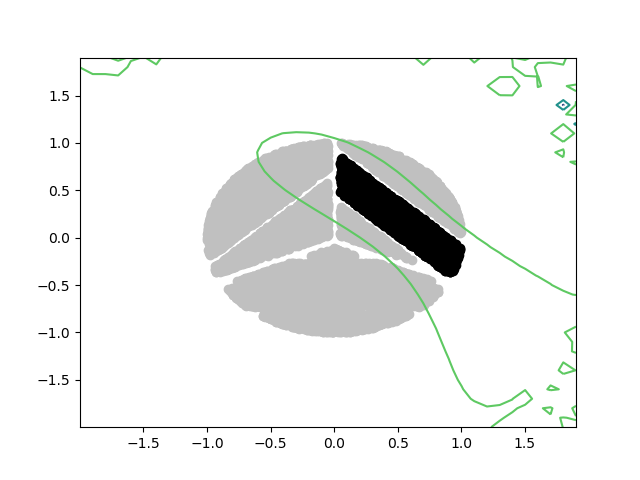
\includegraphics[width=0.5\textwidth]{Figure_6.png}
\caption{
The boundary line of a class (in black) of the kernelized algorithm after $T=10^5$ steps.
}
\label{fig:bound_line2}
\end{figure}

\section{Discussion}